\section{Methods}\label{sec:methods}

My goal with bringing the MLP linked census data
together with the WRA internment camp data
is to create an individual-level panel data set
which includes both those persons who are likely internees
and a control group of people who were almost certainly not interned
(and considered as untreated in the natural experiment of internment).
In a hypothetical experiment with the goal of identifying the causal effect
of forced relocation and incarceration on individual earnings,
a randomly selected set of workers could have been selected from the West Coast
and sent to random destinations in the rest of the US.
In that case, a simple comparison of earnings in the displaced group
against the earnings of the workers on the West Coast who were not interned
would return the causal effect of interest.
Although in some ways Japanese internment does resemble a natural experiment,
there are some important ways in which the way people were actually interned
played out differently than this hypothetical,
which I will address in this section to motivate the main empirical strategy.

Precisely because internment was specifically targeted based on Japanese ancestry,
assignment to treatment was non-random.
\footnote{
  There were several thousand Americans of German and Italian ancestry 
  who were also interned during this period,
  although the overall magnitude was less than the group of Japanese internees
  and much less as a proportion of the existing German and Italian immigrant 
  populations.
  }
If we simply compare interned Japanese earnings after the war
to all other occupants of the West Coast,
then our estimate of internment's effect
will be biased downwards if Japanese were already restricted from
joining certain occupations by discrimination.
One potential comparison group for  West Coast Japanese is Hawaiian Japanese,
who were a large population who were not subject to internment
for economic reasons \citep{chinLongRunLaborMarket2005}.
However, we could expect that Japanese Hawaiians
would have experienced higher growth in their earnings
compared their West Coast peers even without the effect of internment.
The Japanese population in Hawaii were more economically integrated
in especially non-agricultural occupations
and could have experienced less of the post-war anti-Japanese discrimintation.

Another potential comparison group is Japanese living in mainland states 
that were not subject to internment.
However, because such a large proportion of the mainland Japanese population
were living in either Arizona, California, Oregon, or Washington
(about 90\% of the 1940 full-count census data),
this leaves a smaller control group.
Additionally, those Japanese immigrants who had already moved East away
from the point of entry on the West Coast
were likely to already be self-selected individuals
who would have had more access to higher earning job opportunities
due to education or skills.

For the reasons above, 
I follow \cite{arellano-boverDisplacementDiversityMobility2022} 
by including Chinese Americans in my main sample
together with all mainland Japanese.
Chinese immigrants entered the US West Coast 
at a similar period as the major wave of Japanese immigration.
Japanese workers were also seen as a substitute for the cheap Chinese labor 
for work on the transcontinental railroads and in agriculture 
\citep{chenImpactSkillBasedImmigration2015}.
Chinese Americans were not included in any of the relocation 
or internment orders following Executive Order 9066,
but in the absence of internment, 
their wages and employment would likely have continued to evolve similarly 
to the West Coast Japanese population.
For these reasons, Chinese make a natural comparison group 
to recreate the counterfactual earnings outcomes interned Japanese 
would have had if they had never been interned.

Although all persons of Japanese descent living on the West Coast
were ordered to evacuate outside of the Exclusion Area
(and no Chinese persons ordered to evacuate),
the ability of some Japanese to self-evacuate
means some were able to avoid being sent to any of the ten internment camps.
The \cite{dewittjohnl.FinalReportJapanese1943} puts the number of
voluntary evacuees at 4,889.
A research design which treats all Japanese living on the West Coast in 1940
as the treatment group ignore this number
as well as any voluntary emigration by Japanese
out of the West Coast to other states.
In order to estimate a more accurate estimate of the actual
probability that any individual Japanese census respondent was a true internee,
I create a measure of predicted internee status
which uses compares the number of internees in the WRA camp records
against the number of Japanese living in each county in the 1940 census.

\subsection{Predicted Internment Status}\label{sec:data-intern}

The WRA records give a 
(nearly\footnote{Some internees were sent to prisons operated by the 
Department of Justice which were not included in the WRA records.}) 
complete list of all individuals who were interned during World War II.
Although I do not know exactly which of the Japanese individuals 
in the linked sample were those who were actually sent to internment camps,
their original location in 1940 provides a good picture of who would
be likely to be an internee.
Even in the West Coast states which were subjed to internment, 
there was a large amount of variation in the proportion of internees
out of each county's pre-existing Japanese population
as measured in the 1940 full-count census data.

Figure \ref{fig:intern_map} shows a map of all 1940 counties
shaded by the proportion of WRA internees from that county
out of the 1940 Japanese population.
Counties in dark blue had existing Japanese populations in 1940
but for which no residents appear in the internment records.
Counties in yellow had as many (or more) of their 1940 Japanese residents
appear as WRA internees.
Counties which are not shaded did not have any 1940 Japanese residents.

\begin{figure}
  \caption{\label{fig:intern_map} Proportion of 1940 Japanese population interned}
  \begin{adjustbox}{width=\textwidth, center}
    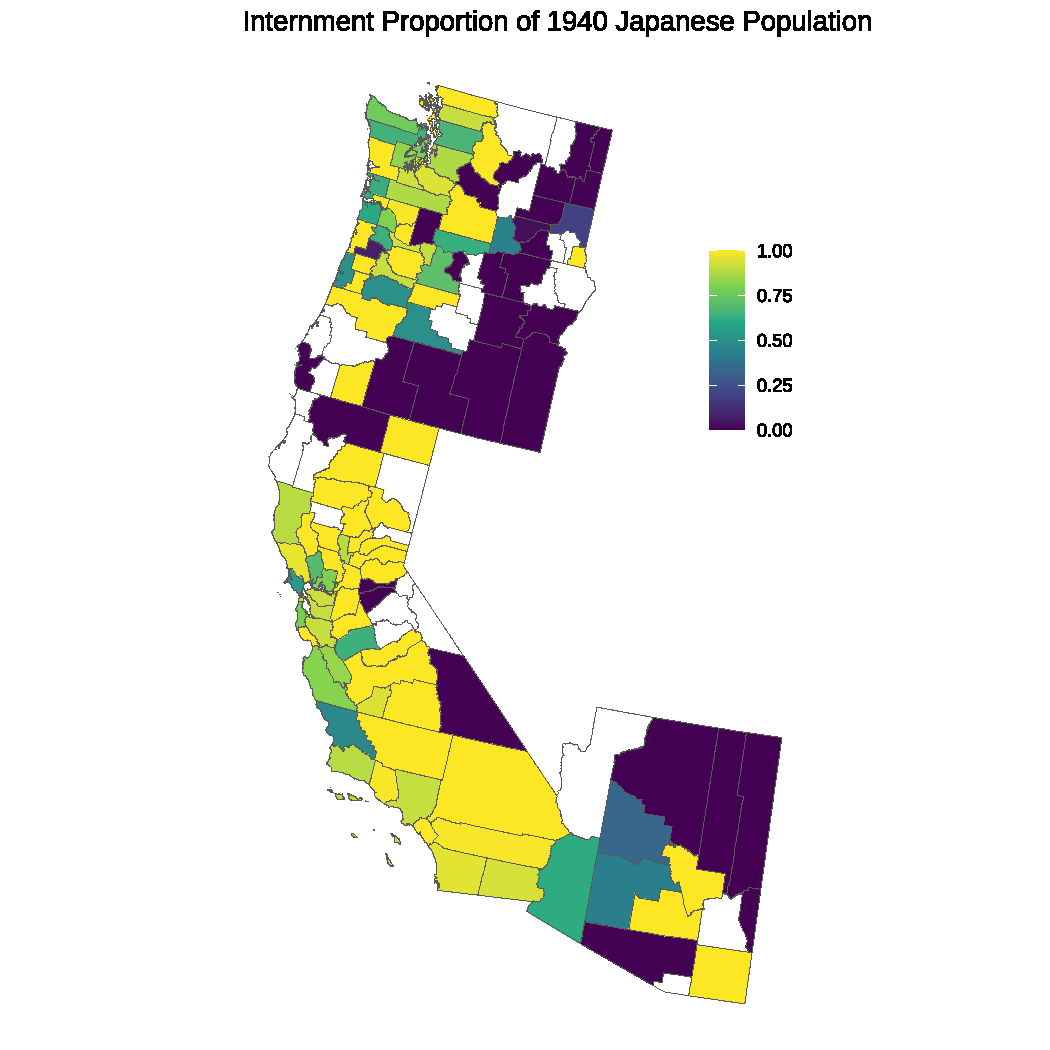
\includegraphics[width=\textwidth]{../figures/pr_interned_map.pdf}
  \end{adjustbox}
  % 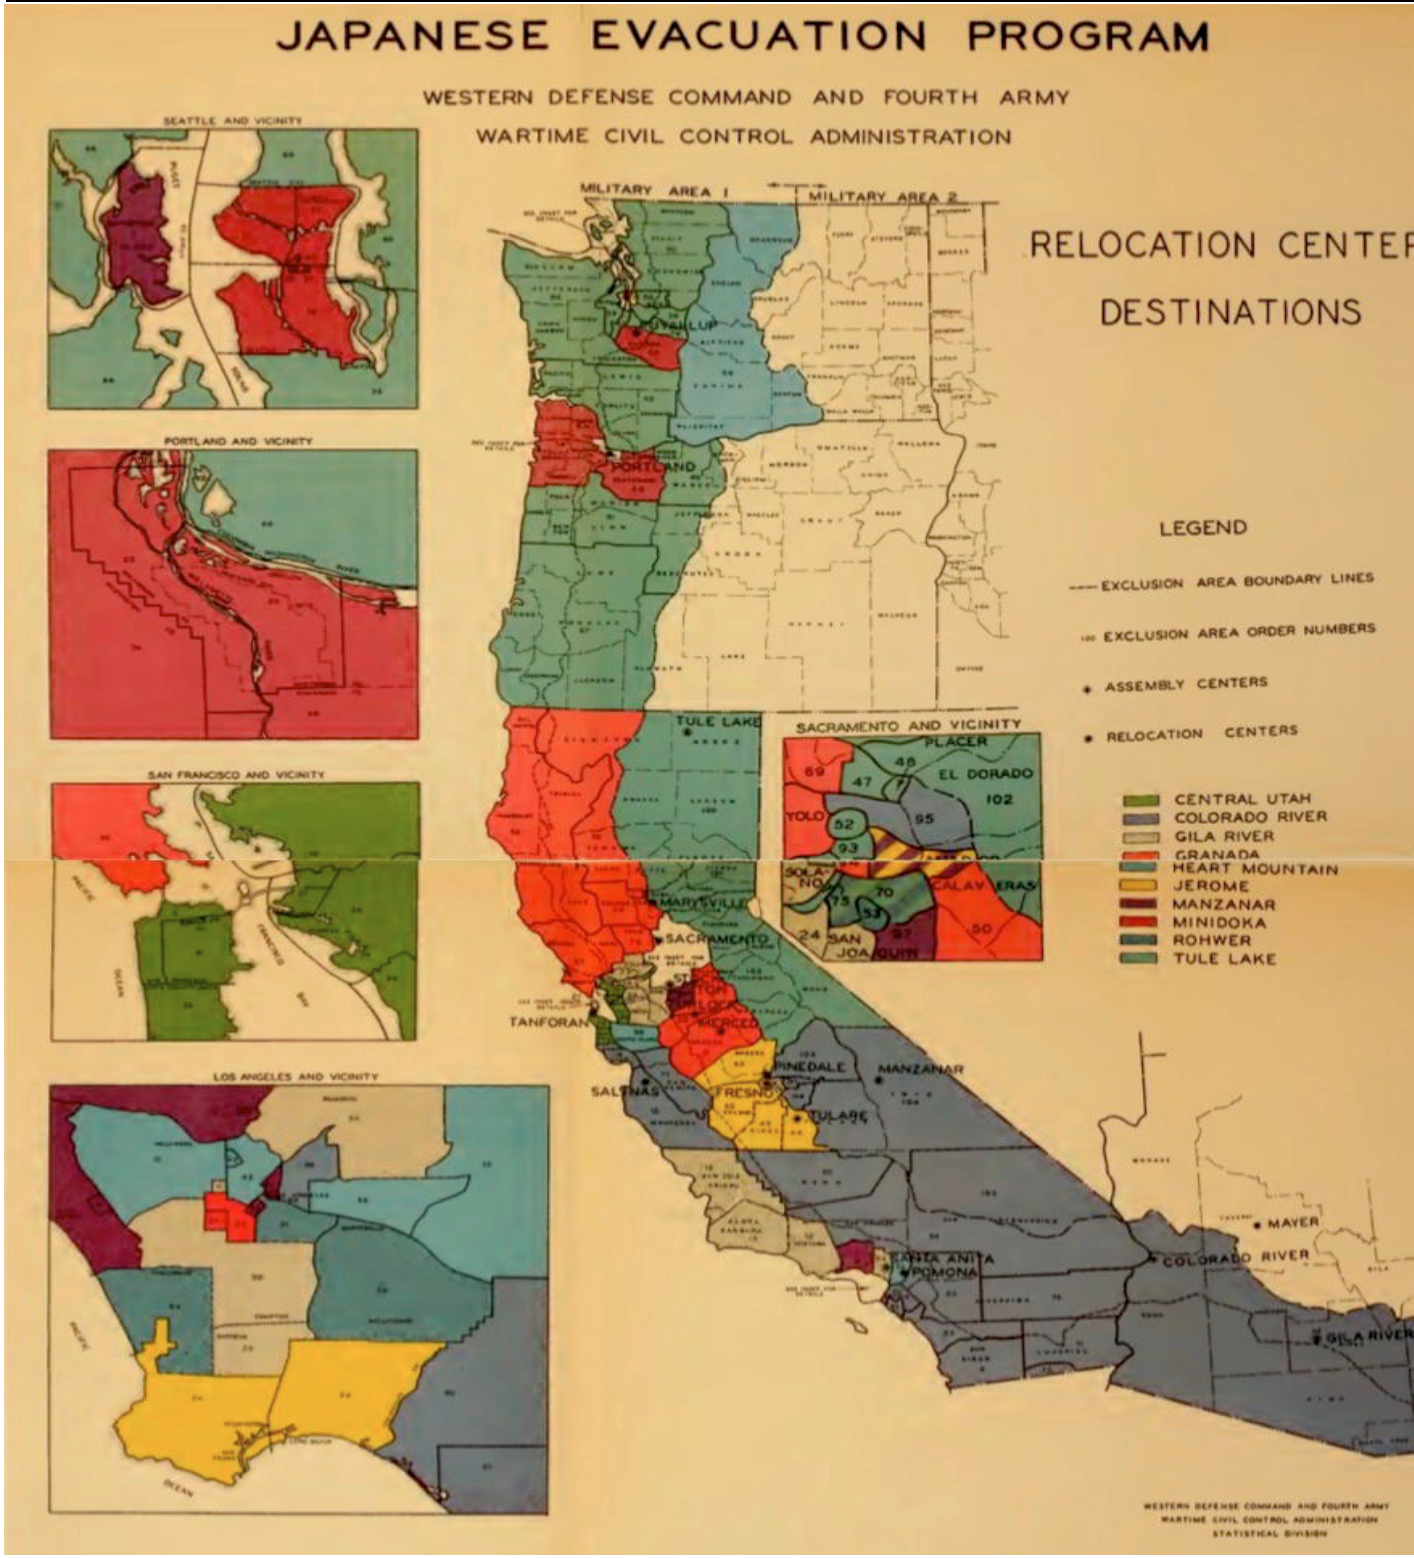
\includegraphics[height=5cm]{../figures/WRAzonesmap.png} \\
  \footnotesize
  Interned proportions are calculated as the number of internees from the county 
  divided by the county's Japanese population in the 1940 full-count census.
  Counties in white had zero Japanese respondents in the 1940 census.
  % The map on the below comes from the 1942 Western Defense Command's Final Report \citep{dewittjohnl.FinalReportJapanese1943}
  % and shows in color the evacuation areas along the West Coast.
\end{figure}


The Exclusion Zone is clearly shown in this map
by the clustering of highly-interned counties in the Southern half of Arizona,
California, and the Western halfs of both Oregon and Washington.
However, based on the comparison between the 1940 census and the WRA records,
it seems like not all counties within the Exclusion Area 
were affected equally.
For example, in San Louis Obisbo County, California,
only 439 of the county's 932 Japanese residents in 1940
ended up in the camp lists.
There are also a few counties outside of the official Exclusion Zone
from which a few internees arrived from
including Curry, New Mexico; Box Elder, Utah; and New York, New York.
This is likely due to either family reunification
or migration from those counties prior to 1942 into the West Coast.

The discrepancy between 1940 Japanese residents and internee origins
could be due to a few reasons.
General demographic changes such as births and deaths
could mean that not everyone who responded to the census was still alive in 1942
or that some children who show up in the internment camps were yet to be born in 1940.
voluntary migration could affect these interned proportions.
Some may have migrated between counties before Pearl Harbor,
or even have chosen to move outside of the Exclusion Zone
during the period when voluntary migration was encouraged by the Army.
If inter-county migration within the West Coast was widespread during this period,
that could mean that some West Coast Japanese who are identified as internees
based on their 1940 county
were actually able to escape the WRA camps.
In this case, it might be more appropriate to interpret the effect of
the predicited internment status estimated here
as the effect of evacuation orders for Japanese overall,
including migration by those who were not actually interned.

% If I move from county A to county B in 1941 and show up in wra from B,
% then I look like I get the treatment effect from county B, not county A

% If the county-level internment proportion is interpreted as 
% effect of forced migration and not camps,
% then voluntary migration outside of the excl zone that was caused by 
% EC9066 doesn't affect causal estimate.
% But if this doesn't matter for causal story,
% then why use county-level stats at all?
% We could just use the evacuation zone as an indicator
% That would treat all west coast Japanese as equally treated.
% Unless we think that voluntary migrants would get a
% different effect of internement than internees

% mention that linked sample doesn't include people who died or left US altogether

Some counties have a proportion greater than one when calculated this way.
For example, one of the thirty counties affected by this is 
Sacramento County in California 
which had a Japanese population of 6,851 in the 1940 census
but in the WRA records there are 7,827 internees who are reported
as coming from Sacramento County.
Although I use this proportion as a measure of internment status
for the linked individuals from each affected county,
it is important to note that this internment status is not a true probability.

% Identifying assumptions
The method of using county-level internment proportions
as a proxy for an individual Japanese worker's own internment status
makes the identifying assumption that
Japanese within the same county had equal chances of being interned.
This would be violated some types of workers were able to avoid internment
for reasons endogenous to their labor market outcomes.
As I discuss in section \ref{sec:history},
voluntary evacuees did anecdotally seem to be more likely relocate
for educational reasons,
or because of family and social networks living out East.
If the types of Japanese who were more likely to be able to voluntarily evacuate
were also more likely to earn higher wages,
then the estimated effect of internment on post-war earnings will
be biased upwards.

To account for this possibility,
I also include an internment status for the linked MLP sample
using the method described in 
\cite{arellano-boverDisplacementDiversityMobility2022}
which conditions on additional demographic variables.
Per his application of Bayes' Rule, 
the probability that an individual $i$ 
in the demographic group $z$ who lived in county $c$ in 1942 was interned
($Pr(I_{i}=1|z_i,c_{i})$)
could be determined from the proportion of the whole population who were interned 
($Pr(I_{i}=1)$,
the proportion of the population with demographics $z$ 
who lived in county $c$ in 1942 ($Pr(z_i,c_{i}^{1942})$),
and the probability of a known internee 
having the same demographics and county in 1942 
($Pr(z_i,c_i^{42}|I_i=1)$).

$$
Pr(I_i=1|z_i,c_i^{42}) = 
\frac{Pr(z_i,c_i^{42}|I_i=1) \cdot Pr(I_i=1)}{Pr(z_i,c_i^{42})}
$$

However, because my target sample of census respondents 
were only asked about their county of residence in the year of the census 
and not in 1942, $c_i^{1940}$ is used as a proxy 
for census respondents' 1942 locations.

The estimator for the true internment status of a census respondent is:

\begin{equation}\label{eq:predint}
\hat{E}[I]_{zc} =
\frac{n(i | z_i=z, ~ c_{i}^{42}=c)}{n(j | z_j=z, ~ c_{j}^{40}=c)}
\end{equation}

This will produce a biased estimate of true internment status if there were unobserved changes in population in each county between 1940 and 1942. For example, for a county that experienced a net outflow of residents, then the ratio of residents in 1940 vs 1942 would be greater than 1 and we would have an estimated internment probability that overstates the likelihood of anyone who lived in that county in 1940 would be interned.

\subsection{Internment's Effect on Earnings}\label{sec:wage-reg}

To measure the effect of internment on earnings, my main analysis follows the following specification:

\begin{equation}\label{eq:mainreg}
  Y_i = \alpha_i + \beta Pr(I)_c + \mathbb{X}_i \Gamma + \epsilon_i
\end{equation}.

The main outcome of interest which I use for $Y_i$ is the reported dollar earnings of individual $i$ in the 1950 census.
$\alpha_i$ represent the state fixed effects for the state in which individual $i$ is living in 1950.
The vector of individual-level controls in $\mathbb{X}$ include age, sex, and individual $i$'s earnings from the 1940 census,
adjusted to 1950 dollars.

The probability of individual $i$ being an internee, $Pr(I)_i$,
is replaced by my estimated version from equation \ref{eq:predint}
using individual $i$'s reported race in 1940 as the only demographic $z$.
The main causal effect of interest is represented by the estimator $\beta$,
which represents the number of dollars of income which an individual is estimated to have gained (or lost)
when going from a non-internee to a likely internee.

A traditional difference-in-differences approach would require the
identifying assumption that both treated and untreated groups
would experience parallel trends in earnings in the absence of internment.
However, if individuals who had pre-existing advantages in the labor market
were able to self-select out of internment through voluntary migration,
then this parallel trends assumption would be violated.
By directly controlling for pre-internment income for each linked individual,
I address this concern for the variables that I do observe consistently
across censuses.

While this empirical strategy does not control 
for all time-invariant unobservable factors,
the historical evidence suggests that
observables like geographic location, education, and pre-war earnings
were the primary factors that determined the ways in which
internment and evacuation policies were individually enforced.
